\chapter{Anforderungsmanagement}
\label{sec:analyse}
%\section{Anforderungsermittlung}
%\subsection{Funktionale Anforderungen}
%\subsection{Systemanforderungen}
%\section{Anforderungsanalyse}
%\section{Anforderungsbeschreibung}
In diesem Kapitel werden die funktionalen Anforderungen für das GuttenBase-Plugin festgelegt. Zunächst werden die Anforderungen grob definiert. Danach werden sie detailliert mithilfe eines vereinfachten Datenmodells beschrieben.

\section{Festlegung der Anforderungen}
%\label{anaylse}
Für die Anforderungsanalyse fanden mehrere Kundengespräche statt. Diese ergaben die folgenden Punkte, die vom GuttenBase-Plugin erfüllt werden sollen:
\begin{itemize}
	\item \textbf{A1: Migrationsoperationen verwalten:}\\
	Um den Migrationsprozess zu individualisieren, soll der Benutzer die Möglichkeit haben, neue Migrationsoperationen zu erstellen, zu editieren und zu löschen.
	\item \textbf{A2: Migrationsoperationen speichern:} \\
	Die hinzugefügten Migrationsoperationen sollen nach der Bestätigung vom Benutzer gespeichert werden können. Sie sollen auch nach einem Neustart der Anwendung zur Verfügung stehen.
	\item \textbf{A3: Überblick über alle Migrationsoperationen:}\\
	Der Benutzer soll über eine tabellarische Auflistung aller erstellten Migrationsoperationen verfügen.
	\item \textbf{A4: Datenbanken verbinden:} \\
	Um eine erfolgreiche Migration durchzuführen, soll der Benutzer in der Lage sein, eine Verbindung zwischen der Quell- und Zieldatenbank herzustellen. Die zu migrierende Datenbank sowie die Zieldatenbank sollen aus den existierenden Datenbanken ausgewählt werden können.
	\item \textbf{A5: Überblick über enthaltene Datenbankelemente:}\\
	Während des Migrationsprozesses soll der Benutzer einen Überblick über alle in der Quelldatenbank enthaltenen Tabellen bzw. Spalten haben.
	\item \textbf{A6: Existierende Migrationsoperationen zur Migration hinzufügen:}\\
	Die gespeicherten Migrationsoperationen sollen in der Übersicht der Datenbankelemente zur Verfügung stehen. Diese können auf die entsprechenden Datenbankelemente angewendet werden.
	\item \textbf{A7: Hinzugefügte Migrationsoperationen löschen}\\	
	Der Benutzer soll die Möglichkeit haben, hinzugefügte Migrationsoperationen zu löschen, nachdem sie zur Migration hinzugefügt worden sind.
	\item \textbf{A8: Migrationsprozess starten} \\
	Im letzten Schritt der Migration kann der Benutzer den Migrationsprozess mit den hinzugefügten Migrationsoperationen starten.	
	\item \textbf{A9: Überblick über den Fortschritt der Migrationsprozesse}\\
	Der Benutzer soll die Möglichkeit haben, hinzugefügte Migrationsoperationen zu löschen, nachdem sie zur Migration hinzugefügt worden sind.
\end{itemize}
Um den Umfang dieser Arbeit in Grenzen zu halten, wurden folgende Migrationsoperationen für die Umsetzung ausgewählt:

\begin{itemize}
	\item Tabellenauswahl,
	\item Spaltenauswahl,
	\item Tabellenumbenennung,
	\item Spaltenumbenennung,
	\item Migrationsfortschritt,
	\item Datentypen der Spalten ändern.
\end{itemize}







\section{Vereinfachtes Datenmodell}
In diesem Abschnitt wird ein vereinfachtes Datenmodell erstellt. Mit diesem wird gezeigt, welche Einheiten des Systems relevant sind und welche Beziehungen zwischen diesen Einheiten gelten. Es handelt sich dabei noch nicht um eine Spezifikation von Klassen für die Implementierung, sondern um eine Modellierung der realen Welt. Das Datenmodell ist maßgebend für die Architektur des Plugins. Aus diesem Grund wird auf unnötige Details bzw. Attribute verzichtet. Das Datenmodell wird als UML-Klassendiagramm in Abbildung 3.1 angegeben. Dabei werden hauptsächlich die Migrationsoperationen und deren Beziehungen dargestellt.
Die abstrakte Klasse ‚GBAction‘ definiert alle möglichen Migrationsoperationen. Sie wird durch die folgenden Unterklassen erweitert:
\begin{itemize}
	\item Rename: \\
	Damit wird das Umbenennen eines Datenbankelementes modelliert. Jede Rename-Klasse hat einen Typ (Rename-Type). Dieser definiert, wie das Umbenennen des Datenbankelementes erfolgen soll und entspricht den in Abschnitt 3.3.0.1 vorgestellten Optionen für das Umbenennen. Außerdem wird die Umbenennung von Spalten bzw. Tabellen in zwei weiteren Unterklassen spezifiziert.
	\item ChangeColumnType: \\
	Diese Klasse entspricht der Migrationsoperation \glqq Datentypen von Spalten ändern\grqq.  
	\item Exclude: \\
	Mit der Exclude-Klasse wird die Migrationsoperation für das Ausschließen einer Spalte bzw. einer Tabelle modelliert.
\end{itemize}
Außerdem enthält die Klasse Migration alle Migrationsoperationen die beim Migrationsprozess angewendet werden.
\begin{figure}[H]
	\centering
	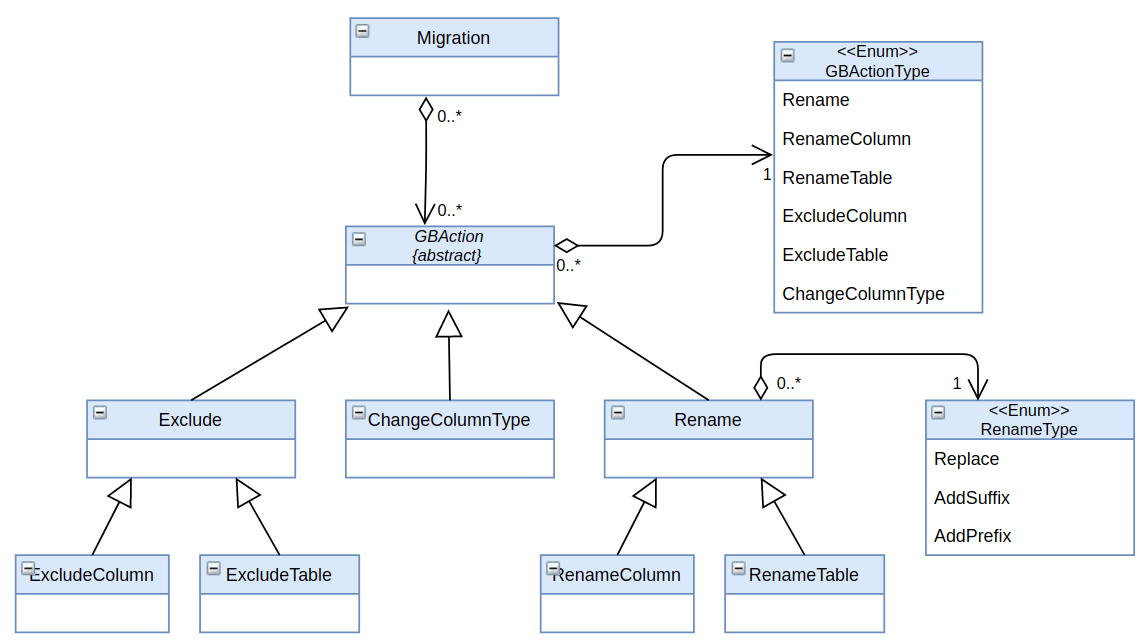
\includegraphics[width=\textwidth]{images/sichten/abstract-datenmodell}
	\caption{Vereinfachtes Datenmodell}
	\label{img:abstract-datenmodell}
\end{figure}


\section{Detaillierte Beschreibung der Anforderungen}
\label{sec:af}
In diesem Abschnitt werden die zu implementierenden Anforderungen behandelt. Diese decken den zentralen Funktionsumfang des Systems ab.
Neben der textuellen Beschreibung werden auch Anwendungsfalldiagramme erstellt. Dabei wird lediglich ein Akteur identifiziert. Dieser ist der Benutzer, der die Datenbankmigration durchführt. Um die Benutzungsführung in den Anwendungsfällen zu illustrieren und die konkrete Benutzeroberfläche, die es zu implementieren gilt, zu spezifizieren, wurden Papierprototypen für die ausschlaggebenden Teile des Systems erzeugt. Diese basieren auf der Norm DIN EN ISO 9241-210.
%todo check norm




\subsubsection{Migrationsoperation: Umbenennen erstellen}
\label{section:umbenennen}
\begin{figure}[H]
	\centering
	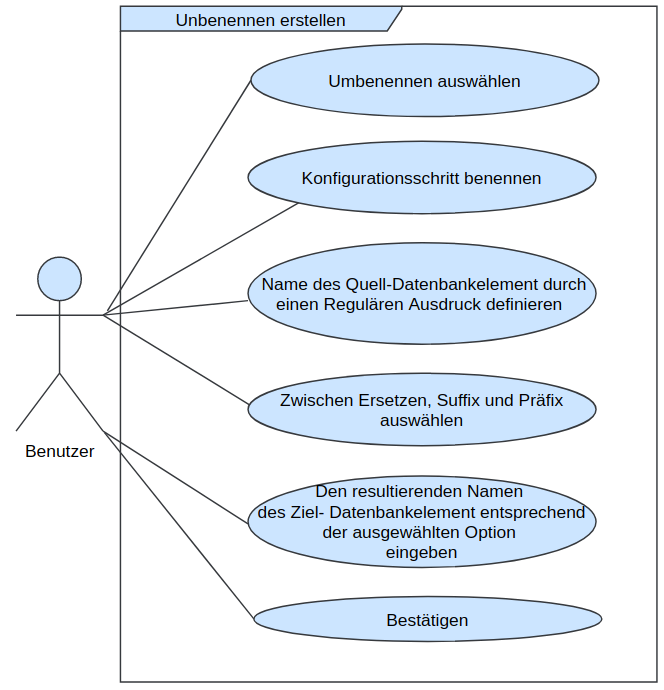
\includegraphics[width=0.7\textwidth]{images/af/af-umbenennen}
	\caption{Migrationsoperation \glqq Umbenennen \grqq erstellen}
	\label{img:af-umbenennen}
\end{figure}
Dieser Anwendungsfall bildet den Vorgang ab, wenn ein Benutzer eine neue Migrationsoperation für das Umbenennen von Spalten bzw. Tabellen in der Zieldatenbank erstellt. Es wird vorausgesetzt, dass der Benutzer die Übersicht aller Migrationsoperationen bereits geöffnet hat (siehe Abbildung \ref{img:actions-overview}). \\
\begin{figure}[H]
	\centering
	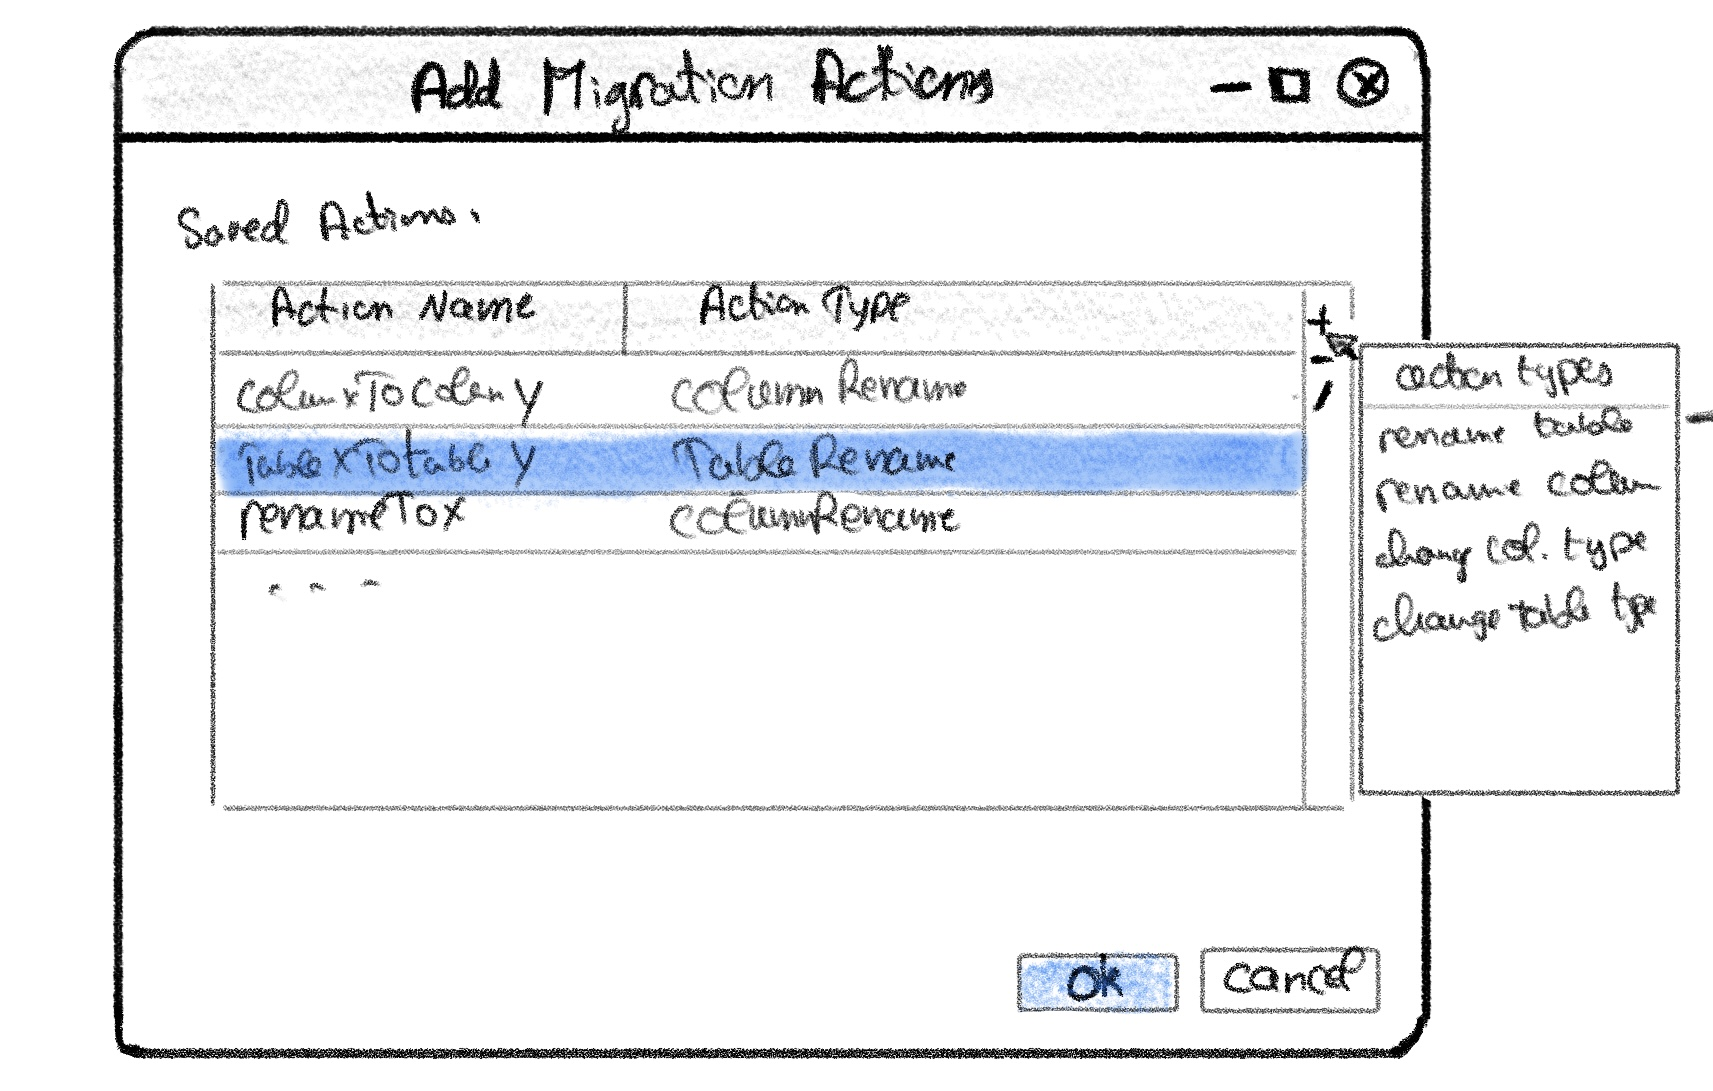
\includegraphics[width=0.5\textwidth]{images/actions-overview}
	\caption{Übersicht Migrationsoperationen}
	\label{img:actions-overview}
\end{figure}
Zu Beginn soll der Benutzer die zu erstellende Migrationsoperation benennen (z. B. ,Rename id to identifier‘). Das Quelldatenbankelement (Spalte oder Tabelle) soll durch einen regulären Ausdruck definiert werden (siehe Abbildung \ref{img:add-rename-action}). Dieser wird in der Migrationsoperation gespeichert, damit er später auf das Datenbankelement angewendet werden kann, das diesen Ausdruck erfüllt. Anschließend wird der Zielname des Datenbankelementes festgelegt. Dieser wird vom Benutzer als eine Zeichenkette angegeben. Dabei stehen drei Optionen zur Verfügung:
\begin{itemize}
	\item \textbf{Ersetzen:} Der vollständige Name des entsprechenden Datenbankelements wird durch die übergebene Zeichenkette ersetzt.
	\item \textbf{Suffix hinzufügen:} Die übergebene Zeichenkette wird als Suffix zum ursprünglichen Namen hinzugefügt.
	\item \textbf{Präfix hinzufügen:} Die übergebene Zeichenkette wird als Präfix zum ursprünglichen Namen hinzugefügt.
\end{itemize}
\begin{figure}[H]
	\centering
	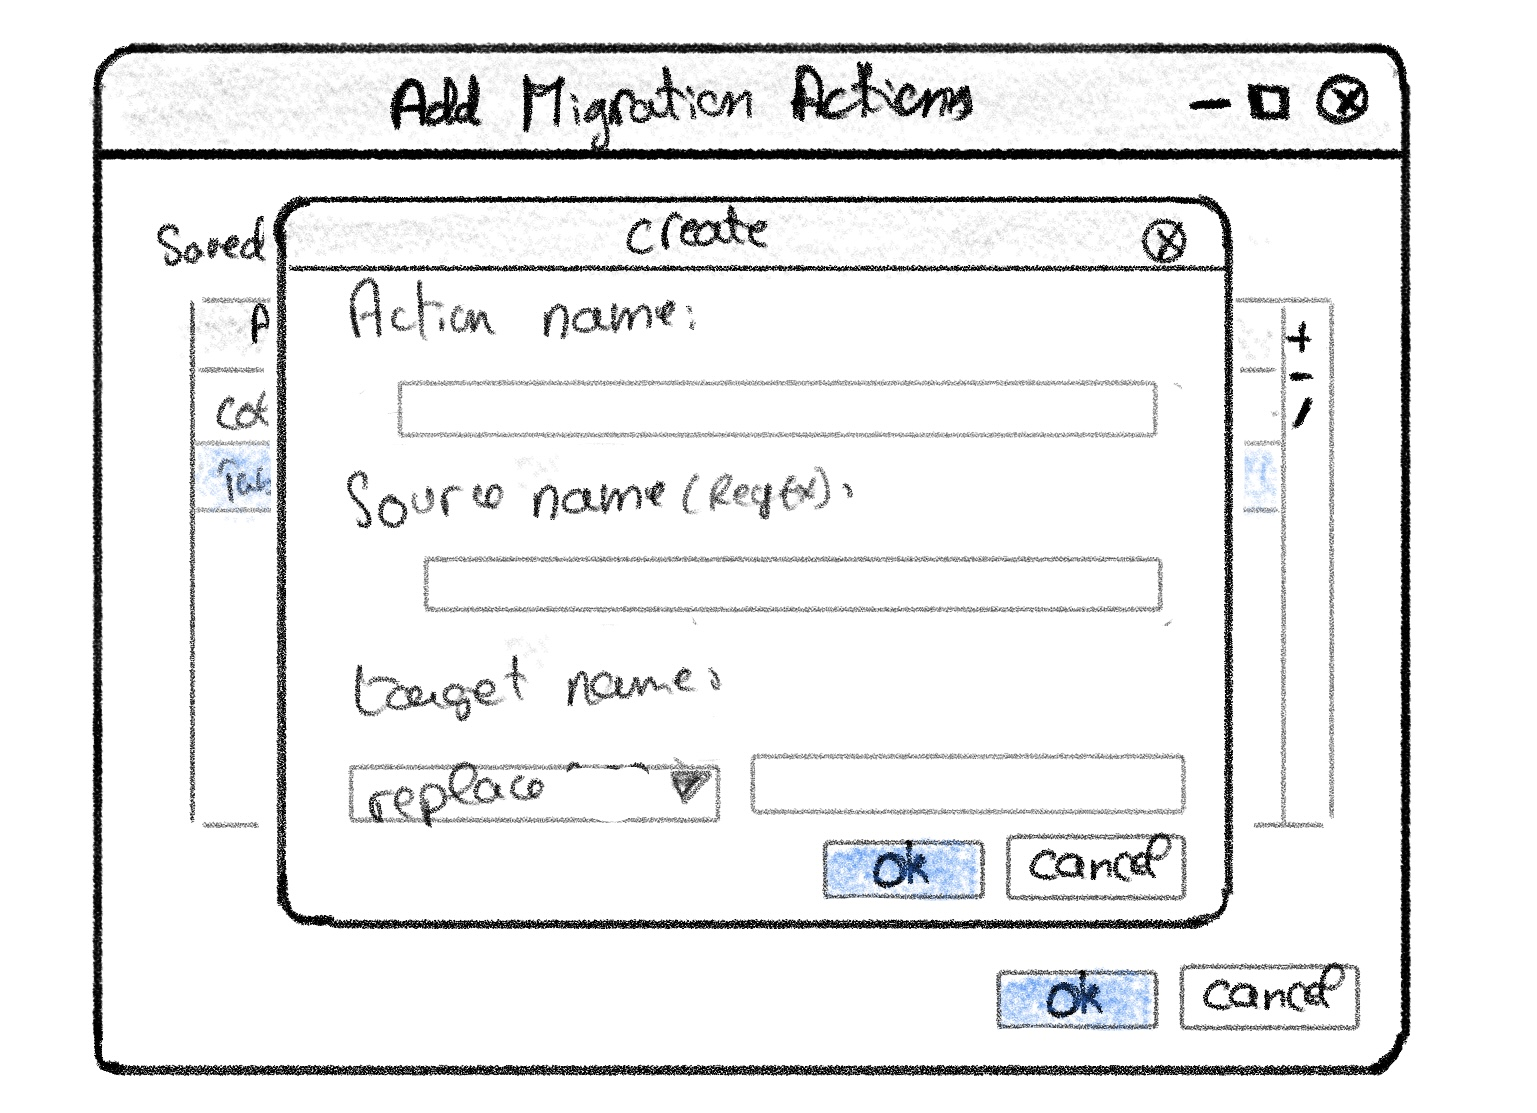
\includegraphics[width=0.5\textwidth]{images/add-rename-action}
	\caption{Migrationsoperation: Umbenennen}
	\label{img:add-rename-action}
\end{figure}
Nach dem Bestätigen der Eingaben wird die neu erstellte Migrationsoperation der Liste aller Migrationsoperationen hinzugefügt.
\begin{table}[H]
	\centering
	\caption{Anwendungsfall: Migrationsoperation Umbenennen erstellen}
	\begin{tabular}{ |p{4cm}|p{8cm}| }
		\hline
		\textbf{Name} &  Migrationsoperation Umbenennen erstellen \\
		\hline
		\textbf{Akteure} & Benutzer \\
		\hline
		\textbf{Auslöser} & Der Nutzer ist in der Übersicht der Migrationsoperationen und hat auf den \glqq $+$\grqq Button geklickt. \\
		\hline
		\textbf{Vorbedingung} & Der Nutzer besitzt eine List von Migrationsoperationen.  \\
		\hline
		\textbf{Nachbedingung} & Eine Migrationsoperation vom Typ Umbenennen wird zur Liste aller Migrationsoperationen hinzugefügt.  \\
		\hline
		\textbf{Ablauf} & 
		\begin{enumerate}
			\item Die Option \glqq Umbenennen\grqq auswählen.
			\item Einen Namen für die zu erstellende Migrationsoperation eingeben.
			\item Den Namen des Quelldatenbankelement durch einen regulären Ausdruck definieren.
			\item Zwischen Ersetzen, Suffix und Präfix auswählen.
			\item Den resultierenden Namen des Ziedatenbankelements entsprechend der ausgewählten Option eingeben.
			\item Bestätigen.
		\end{enumerate}  \\
		\hline
		
	\end{tabular}
	\label{table:umbenennen}
\end{table}




\subsubsection{Migrationsoperation erstellen: Datentyp ändern }
\begin{figure}[H]
	\centering
	\includegraphics[width=0.7\textwidth]{images/af/af-datentyp-ändern}
	\caption{Migrationsoperation \glqq Datentyp ändern \grqq erstellen}
	\label{img:af-datentyp-ändern}
\end{figure}

Dieser Anwendungsfall zeigt, wie der Benutzer die Migrationsoperation ,Datentyp ändern‘ erstellt. Wie beim vorangegangenen Anwendungsfall soll sich der Benutzer in der Übersicht über alle Migrationsoperationen befinden, um in den Anwendungsfall einzutreten (siehe Abbildung \ref{img:actions-overview}).\\
Nach dem Auslösen des Anwendungsfalls soll der Benutzer die Option ‚Datentyp ändern‘ auswählen. Danach hat der Benutzer die Möglichkeit, die Migrationsoperation zu benennen, den Datentyp der Quelldatenbank bzw. der Zieldatenbank als Zeichenkette einzugeben und anschließend die Eingaben zu bestätigen. Nachdem dieser Anwendungsfall beendet worden ist, wird eine neue Migrationsoperation hinzugefügt.\\ \\
Das Erstellen der Migrationsoperation ‚Exkludieren‘ funktioniert ähnlich wie die zwei vorherigen Anwendungsfälle und wird daher nicht behandelt.
\begin{table}[H]
	\centering
	\caption{Anwendungsfall: Migrationsoperation ,Datentyp ändern‘ erstellen}
	\begin{tabular}{ |p{4cm}|p{8cm}| }
		\hline
		\textbf{Name} &  Migrationsoperation Datentyp ändern erstellen \\
		\hline
		\textbf{Akteure} & Benutzer  \\
		\hline
		\textbf{Auslöser} & Der Nutzer ist in der Übersicht der Migrationsoperationen und hat auf den ,+‘-Button geklickt. \\
		\hline
		\textbf{Vorbedingung} & Der Nutzer besitzt eine List von Migrationsoperationen.  \\
		\hline
		\textbf{Nachbedingung} & Eine Migrationsoperation vom Typ ,Datentyp ändern‘ wird zur Liste aller Migrationsoperationen hinzugefügt.  \\
		\hline
		\textbf{Ablauf} & 
		\begin{enumerate}
			\item Die Option ,Datentyp ändern‘ auswählen
			\item Einen Namen für die zu erstellende Migrationsoperation eingeben
			\item Den Datentyp der Quellspalte festlegen
			\item Den Datentyp der Zielspalte eingeben
			\item Bestätigen
		\end{enumerate}   \\
		\hline
		
	\end{tabular}
	\label{table:datentyp-ändern}
\end{table}

\subsubsection{Migrationsoperationen verwalten}
\begin{figure}[H]
	\centering
	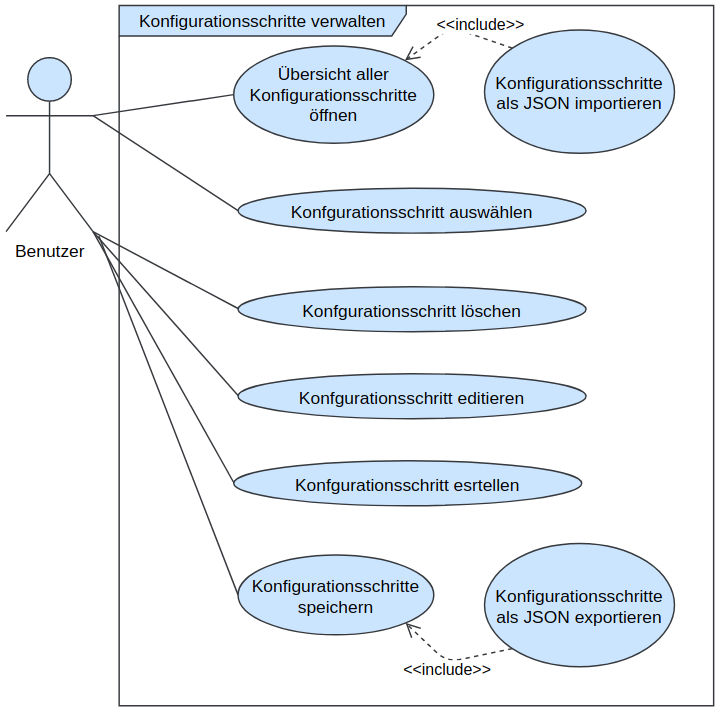
\includegraphics[width=0.7\textwidth]{images/af/af-ks-verwalten}
	\caption{Migrationsoperationen verwalten}
	\label{img:af-ks-verwalten}
\end{figure}

Dieser Anwendungsfall beinhaltet die Verwaltung der Migrationsoperationen. Zunächst soll der Benutzer die Übersicht der Migrationsoperationen öffnen (siehe Abbildung \ref{img:actions-overview}). Dabei werden alle gespeicherten Migrationsoperationen geladen. Diese werden aus einer JSON-Datei erzeugt.\\ In der Übersicht kann der Benutzer einzelne oder mehrere Migrationsoperationen zugleich löschen. Außerdem kann er Migrationsoperationen erstellen (Dieser Vorgang wurde in den vorangegangenen Anwendungsfällen beschrieben). Das Editieren der Migrationsoperationen erfolgt ebenso wie das Erstellen.\\
Anschließend können die Migrationsoperationen nach der Bestätigung durch den Benutzer als JSON gespeichert werden.
\begin{table}[H]
	\centering
	\caption{Anwendungsfall Migrationsoperationen verwalten}
	\begin{tabular}{ |p{4cm}|p{8cm}| }
		\hline
		\textbf{Name} & Migrationsoperationen verwalten  \\
		\hline
		\textbf{Akteure} &  Benutzer \\
		\hline
		\textbf{Auslöser} &  Der Benutzer klickt auf einen Button, um die Übersicht aller Migrationsoperationen zu sehen. \\
		\hline
		\textbf{Vorbedingung} & Der Benutzer verfügt über eine initiale Liste der Migrationsoperationen.  \\
		\hline
		\textbf{Nachbedingung} & Die Änderungen sind vorgenommen und gespeichert.  \\
		\hline
		\textbf{Ablauf} & 
		\begin{enumerate}
			\item Übersicht aller Migrationsoperationen öffnen.
			\item eventuell Migrationsoperationen auswählen.
			\item eventuell Migrationsoperationen löschen.
			\item eventuell eine Migrationsoperation editieren.
			\item eventuell eine Migrationsoperation erstellen.
			\item Migrationsoperationen speichern.
		\end{enumerate}   \\
		\hline
		
	\end{tabular}
	\label{table:ks-speichern}
\end{table}



\subsubsection{Datenbankmigration durchführen}
Die Durchführung der Datenbankmigration deckt die Hauptfunktionalität des GuttenBase-Plugins ab. Die Migration wird in die folgenden Anwendungsfälle unterteilt:
\subsubsection*{Datenbanken verbinden}
\begin{figure}[H]
	\centering
	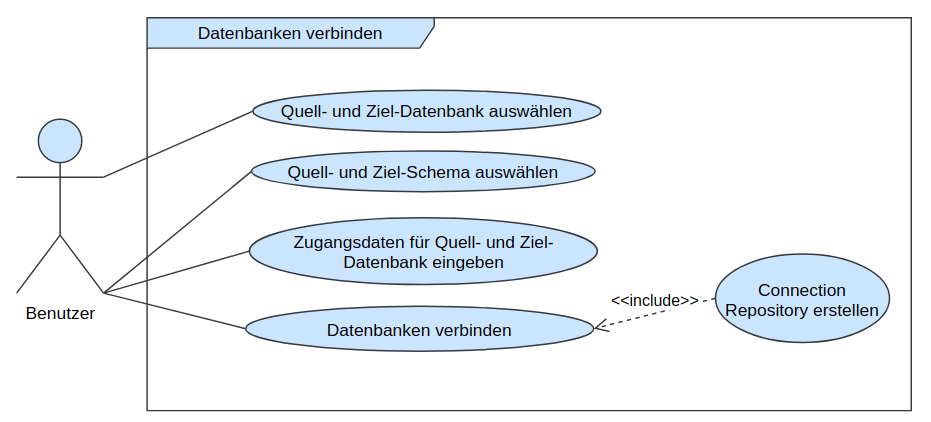
\includegraphics[width=0.7\textwidth]{images/af/af-db-verbinden}
	\caption{Datenbanken verbinden}
	\label{img:af-db-verbinden}
\end{figure}

Für das Eintreten dieses Anwendungsfalls wird vorausgesetzt, dass der Benutzer über mindestens eine Datenbank verfügt. Zu Beginn muss er das Migrationsfenster öffnen, um die Eingabefelder zu sehen. Anschließend soll er die Datenbank, das Schema sowie die Zugangsdaten für das Quell- und Ziel-DBMS angeben (siehe Abbildung \ref{img:generalview}). 
Wenn die Eingaben stimmen, kann der Benutzer eine Verbindung zwischen den beiden Datenbanken herstellen. Ansonsten wird eine entsprechende Meldung angezeigt. Bei diesem Schritt wird das Connector-Repository der GuttenBase-Bibliothek erstellt und konfiguriert. Somit ist die Datenbankmigration bereit für die Konfiguration.
\begin{figure}[H]
	\centering
	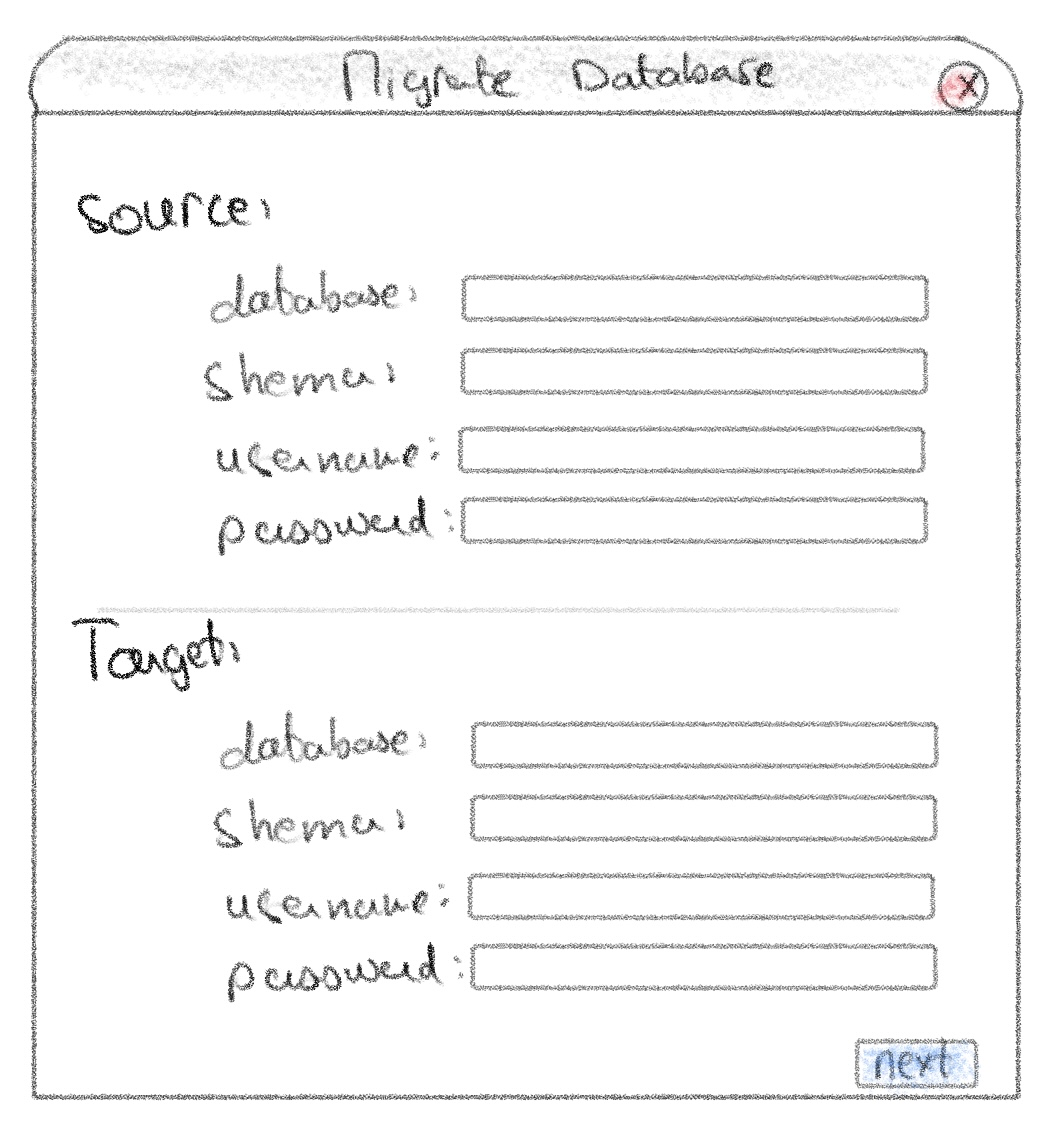
\includegraphics[width=0.5\textwidth]{images/generalview}
	\caption{Datenbankmigration View}
	\label{img:generalview}
\end{figure}
\begin{table}[H]
	\centering
	\caption{Anwendungsfall Datenbanken verbinden}
	\begin{tabular}{ |p{4cm}|p{8cm}| }
		\hline
		\textbf{Name} & Datenbanken verbinden  \\
		\hline
		\textbf{Akteure} & Benutzer  \\
		\hline
		\textbf{Auslöser} & Der Benutzer klickt auf einen Button um die Übersicht der Datenbankverbindung zu öffnen. \\
		\hline
		\textbf{Vorbedingung} & Die Quell- und Zieldatenbanken sind nicht mit dem GuttenBase-Tool verbunden.\\
		\hline
		\textbf{Nachbedingung} & Die Quell- und Zieldatenbanken sind verbunden.  \\
		\hline
		\textbf{Ablauf} &  
		\begin{enumerate}
			\item Quelldatenbank auswählen
			\item Quellschema auswählen
			\item Benutzername der Quelldatenbank eingeben
			\item Passwort der Quelldatenbank eingeben
			\item Zieldatenbank auswählen
			\item Zielschema auswählen
			\item Benutzername der Zieldatenbank eingeben
			\item Passwort der Zieldatenbank eingeben
			\item Datenbanken verbinden
		\end{enumerate}  \\
		\hline
		
	\end{tabular}
	\label{table:db-verbinden}
\end{table}


\subsubsection*{Migrationsprozess konfigurieren}
\begin{figure}[H]
	\centering
	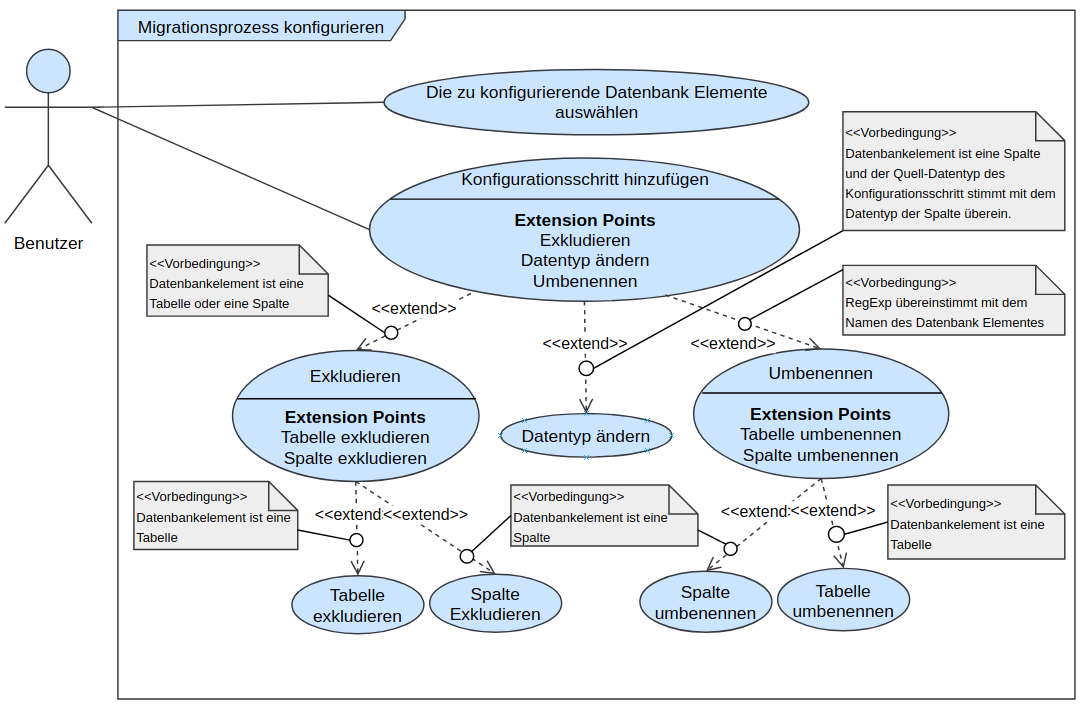
\includegraphics[width=0.9\textwidth]{images/af/af-mg-cfg}
	\caption{Migrationsprozess konfigurieren}
	\label{img:af-mg-cfg}
\end{figure}

Dieser Anwendungsfall zeigt den Vorgang, wie der Benutzer Migrationsoperationen zum Migrationsprozess hinzufügen kann.\\
Es wird vorausgesetzt, dass die Quell- und Zieldatenbanken verbunden sind (siehe Anwendungsfall \ref{table:db-verbinden})\\
Wenn der Nutzer auf ,Next‘ geklickt hat, soll eine Übersicht für alle in der Quelldatenbank enthaltenen Elemente angezeigt werden (Siehe Abbildung \ref{img:overview}).
\begin{figure}[H]
	\centering
	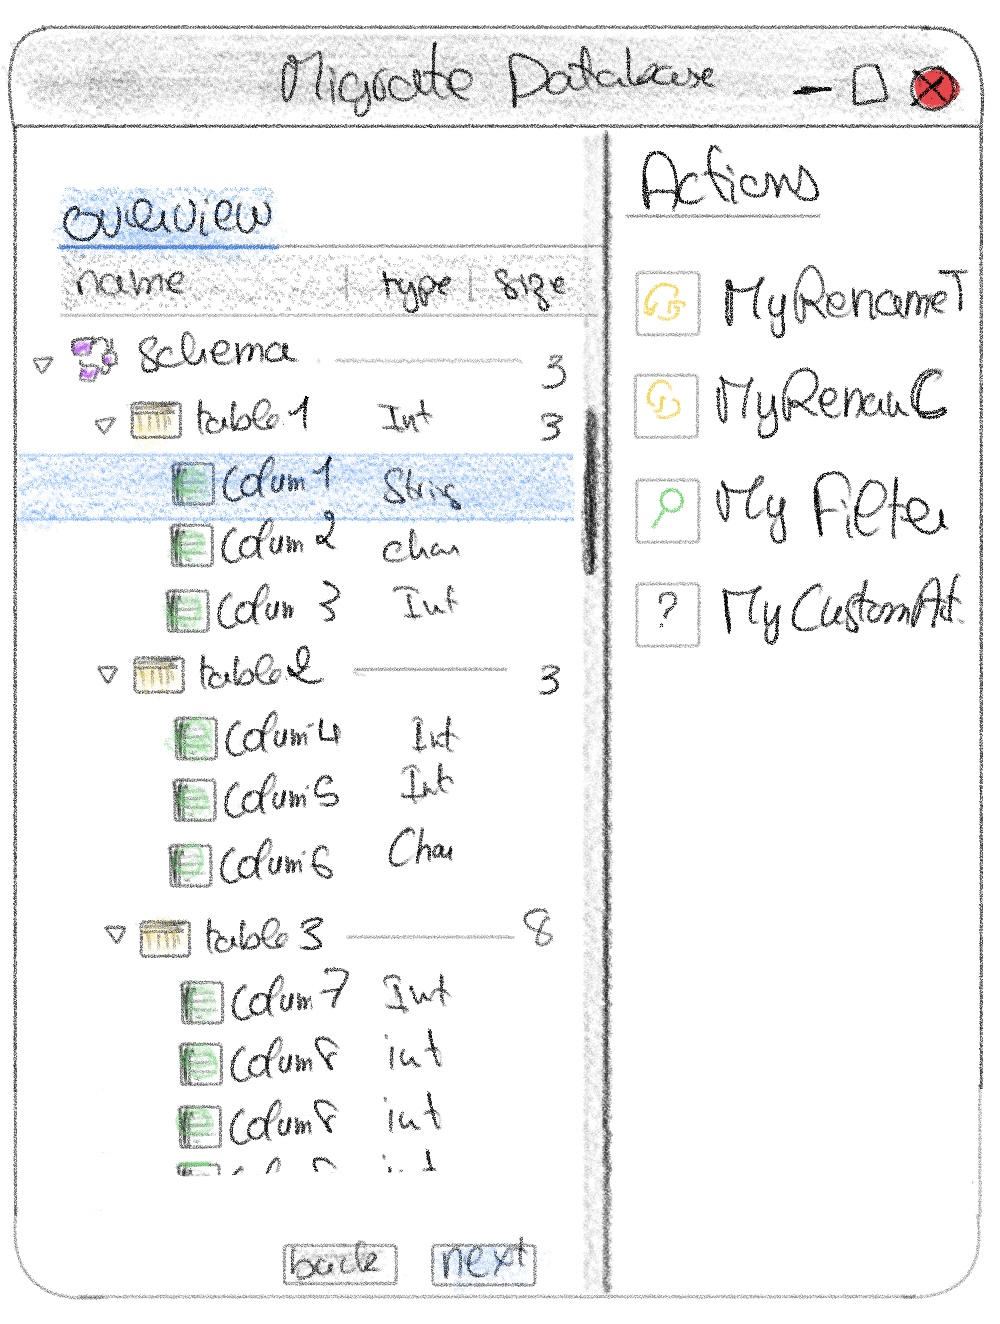
\includegraphics[width=0.5\textwidth]{images/overview}
	\caption{Übersicht Quelldatenbank}
	\label{img:overview}
\end{figure}
Der Benutzer kann zunächst Spalten bzw. Tabellen auswählen, um diesen Migrationsoperationen zuzuweisen.\\
Je nachdem wie die Auswahl der Datenbankelemente aussieht, stehen lediglich passende Migrationsoperationen zur Verfügung. Um eine Tabelle bzw. eine Spalte zu exkludieren, ist es ausreichend, wenn das selektierte Datenbankelement eine Tabelle bzw. eine Spalte ist.\\
Weiter wird beim Hinzufügen der Migrationsoperation ‚Datentyp ändern‘ geprüft, ob die ausgewählten Datenbankelemente Spalten sind und ob deren Datentypen dem Datentyp der Migrationsoperation entsprechen.\\
Außerdem wird beim Umbenennen der ausgewählten Tabellen bzw. Spalten kontrolliert, ob die Namen mit dem in der Migrationsoperation gespeicherten regulären Ausdruck übereinstimmen. \\
Nachdem der Benutzer alle gewünschten Migrationsoperationen ausgewählt hat, werden diese gespeichert und zum Migrationsprozess hinzugefügt.

\begin{table}[H]
	\centering
	\caption{Anwendungsfall Migrationsprozess konfigurieren}
	\begin{tabular}{ |p{4cm}|p{8cm}| }
		\hline
		\textbf{Name} &  Migrationsprozess konfigurieren. \\
		\hline
		\textbf{Akteure} & Benutzer  \\
		\hline
		\textbf{Auslöser} & Der Benutzer klickt auf den ,Next‘-Button.  \\
		\hline
		\textbf{Vorbedingung} &  Die Migration ist nicht konfiguriert. \\
		\hline
		\textbf{Nachbedingung} &  Die Migration ist nach den Wünschen des Benutzers konfiguriert. \\
		\hline
		\textbf{Ablauf} & 
		\begin{enumerate}
			\item Die zu konfigurierenden Datenbankelemente auswählen
			\item Migrationsoperation hinzufügen (dieser Schritt kann mehrmals durchgeführt werden)
		\end{enumerate}   \\
		\hline
		
	\end{tabular}
	\label{table:migration-cfg}
\end{table}



\subsubsection*{Hinzugefügte Migrationsoperationen löschen}	
\begin{figure}[H]
	\centering
	\includegraphics[width=0.7\textwidth]{images/af/af-ks-löschen}
	\caption{Hinzugefügte Migrationsoperationen löschen}
	\label{img:af-ks-löschen}
\end{figure}
Das Löschen einer hinzugefügten Migrationsoperation ist erst möglich, wenn sich der Benutzer in der entsprechenden Übersicht befindet (siehe Abbildung \ref{img:result-view}). Dabei werden alle hinzugefügten Migrationsoperationen aufgelistet.Diese können ausgewählt und anschließend gelöscht werden.
\begin{figure}[H]
	\centering
	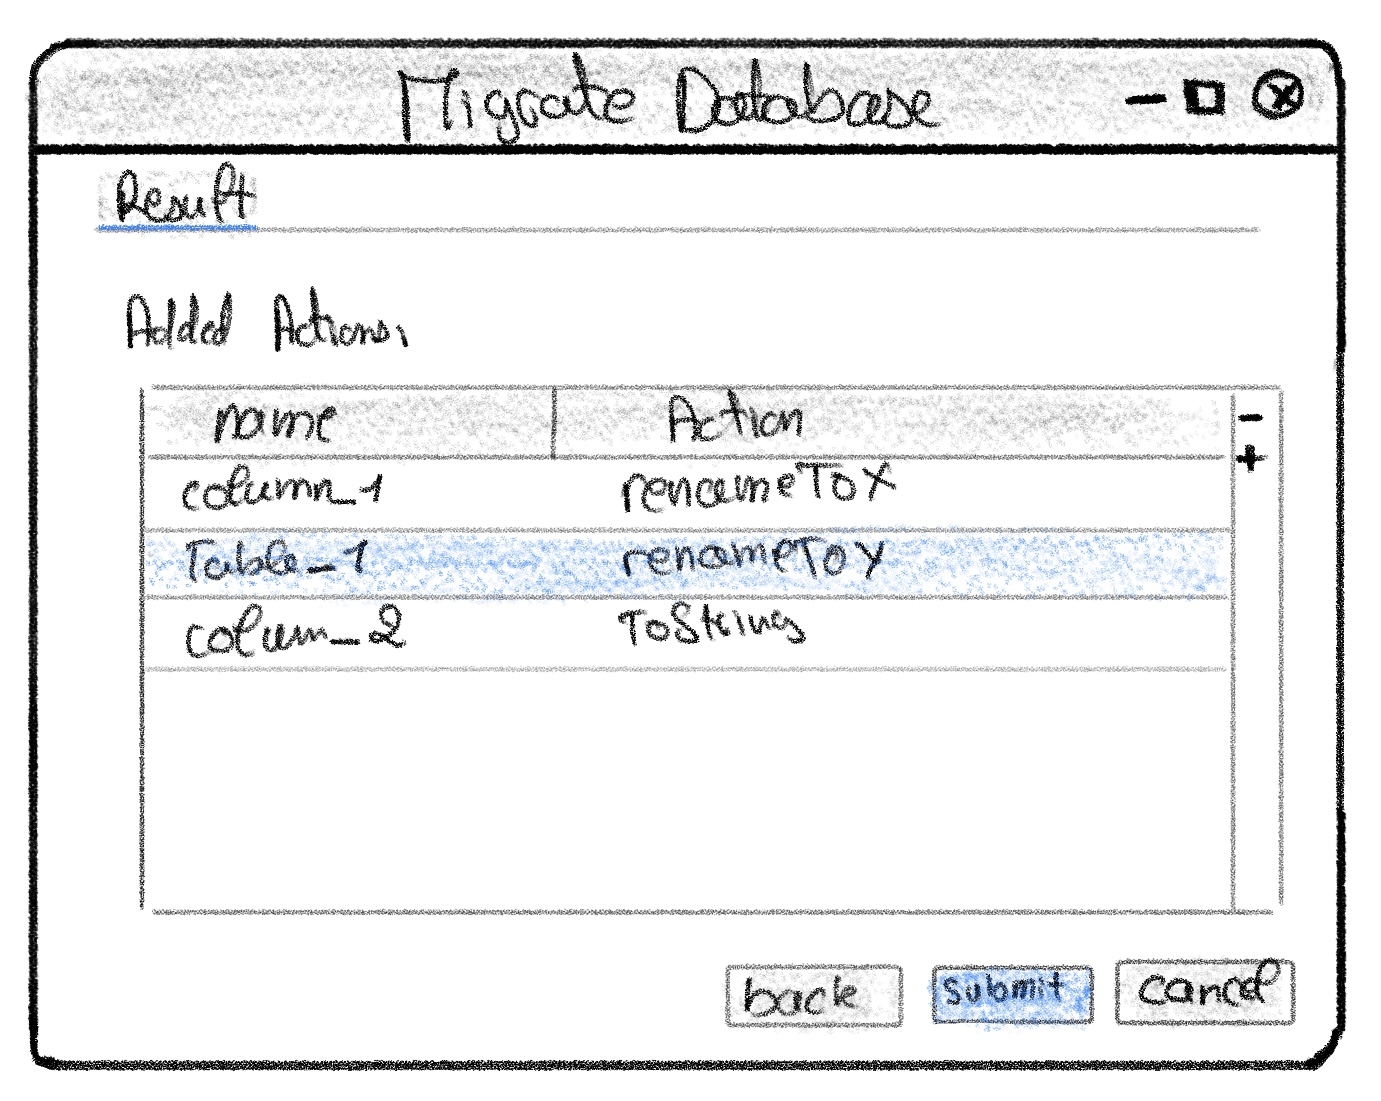
\includegraphics[width=0.6\textwidth]{images/result-view}
	\caption{Übersicht über die hinzugefügten Migrationsoperationen}
	\label{img:result-view}
\end{figure}
\begin{table}[H]
	\centering
	\caption{Anwendungsfall Anwendungsfall ,hinzugefügte Migrationsoperationen löschen‘}
	\begin{tabular}{ |p{4cm}|p{8cm}| }
		\hline
		\textbf{Name} &  Hinzugefügte Migrationsoperationen löschen. \\
		\hline
		\textbf{Akteure} &  Benutzer. \\
		\hline
		\textbf{Auslöser} & Der Benutzer klickt auf den ,Next‘-Button. \\
		\hline
		\textbf{Vorbedingung} & Die hinzugefügten Migrationsoperationen sind nicht gelöscht.  \\
		\hline
		\textbf{Nachbedingung} &  Die hinzugefügten Migrationsoperationen sind gelöscht. \\
		\hline
		\textbf{Ablauf} &  
		\begin{enumerate}
			\item Die zu löschenden Migrationsoperationen auswählen
			\item Die ausgewählten Migrationsoperationen löschen
		\end{enumerate}  \\
		\hline
		
	\end{tabular}
	\label{table:migration-ks-löschen}
\end{table}



\subsubsection*{Migration starten}
\begin{figure}[H]
	\centering
	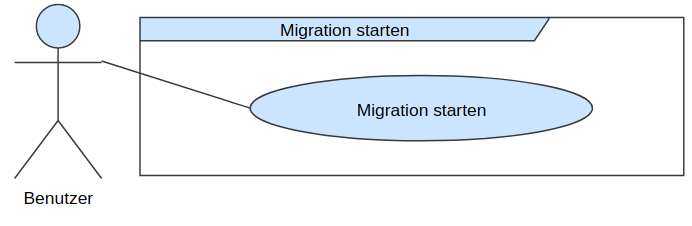
\includegraphics[width=0.7\textwidth]{images/af/af-mg-starten}
	\caption{Migration starten}
	\label{img:af-mg-starten}
\end{figure}
Nachdem der Benutzer alle Datenbanken verbunden und den Migrationsprozess konfiguriert hat, kann er die Migration der Datenbank durch eine einfache Bestätigung starten. Danach sollen die Daten entsprechend der Konfiguration migriert werden. Währenddessen soll der Benutzer über den Migrationsstand informiert werden (siehe Abbildung \ref{img:progressview}).
\begin{figure}[H]
	\centering
	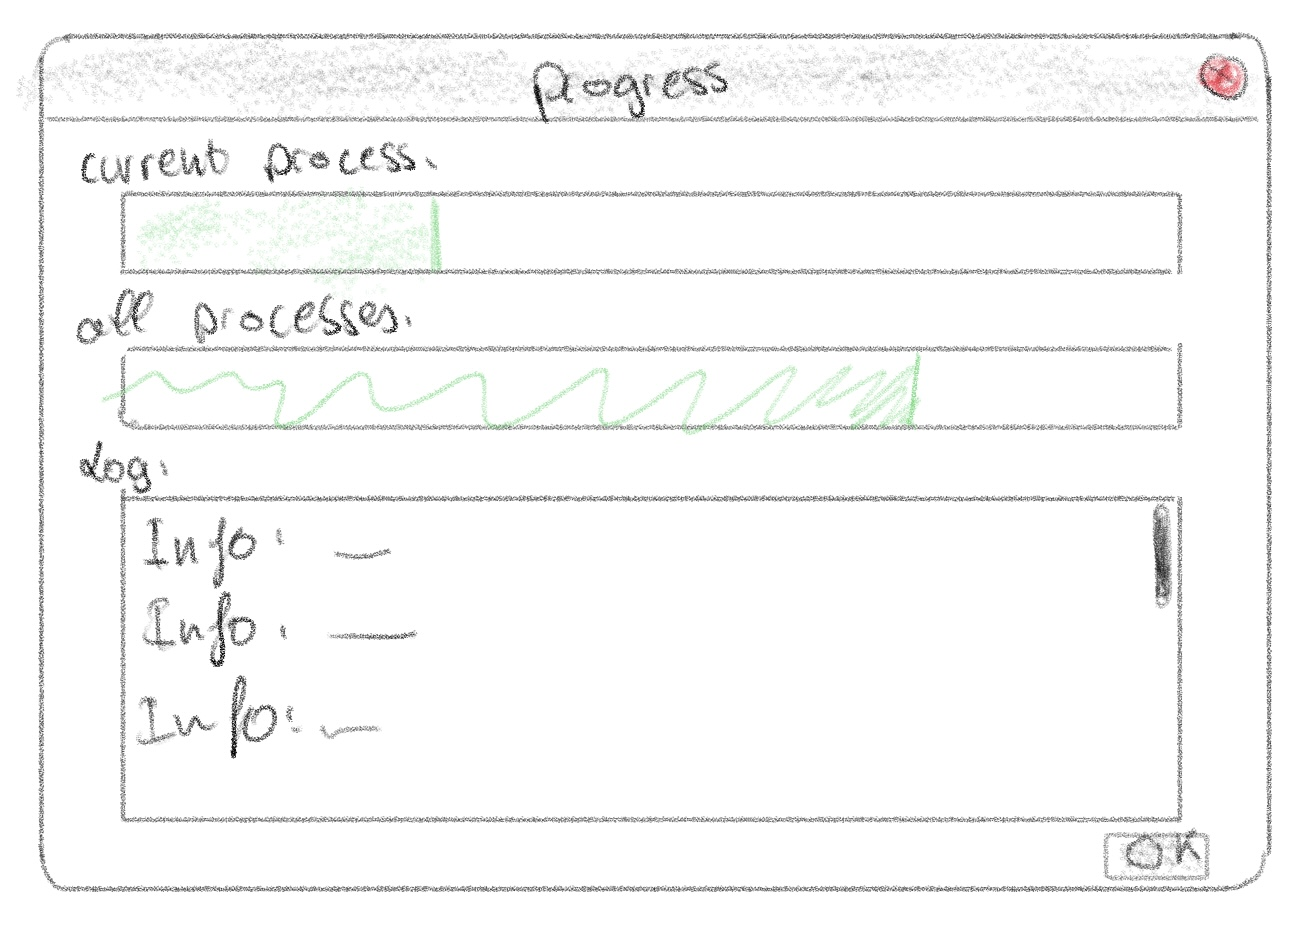
\includegraphics[width=0.4\textwidth]{images/progressview}
	\caption{Fortschritt des Migrationsprozesses}
	\label{img:progressview}
\end{figure}
\begin{table}[H]
	\centering
	\caption{Anwendungsfall Migration starten}
	\begin{tabular}{ |p{4cm}|p{8cm}| }
		\hline
		\textbf{Name} & Migration starten  \\
		\hline
		\textbf{Akteure} & Benutzer  \\
		\hline
		\textbf{Auslöser} & Der Benutzer klickt auf den ,Migrieren‘-Button. \\
		\hline
		\textbf{Vorbedingung} & Die Quelldatenbank ist noch nicht migriert.  \\
		\hline
		\textbf{Nachbedingung} & Die Quelldatenbank ist migriert.  \\
		\hline
		\textbf{Ablauf} &  
		\begin{enumerate}
			\item Migration starten.
		\end{enumerate}  \\
		\hline
		
	\end{tabular}
	\label{table:migration-starten}
\end{table}

%\subsection{Probleme und Strategien}
%- Umsetzungsform\\
%- ...

